\section{Analyse Technique}

\subsection{Présentation}

\subsubsection{Histoire de l'analyse technique}
Les sources de l'analyse technique remonte au XVIIIème siècle quand les Japonais essayaient d'anticiper l'évolution des cours du riz. Ensuite, on retrouve trace de l'analyse technique au début du XXème siècle grâce aux recherches de Richard Dow. Au début, l'analyse technique était purement graphique mais désormais on retrouve une grande part d'outil mathématiques. \\

A partir des années 30, Ralph Nelson Elliot a mis en évidence les fameuses vagues d'Elliot. Nous retrouvons également d'autres grands noms associés à l'analyse technique tels que Steve Nison, réputé pour la méthode des chandeliers, Stan Weinstein, pour les moyennes mobiles et John Bollinger. \\


\subsubsection{Définition}
Tentant de définir l’analyse technique, John Murphy disait : « L’analyse technique est l’étude de l’évolution d’un marché, principalement sur la base de graphiques, dans le but de prévoir les futures tendances ». L'analyse technique correspond à l'étude des graphiques des cours de la bourse ainsi que de divers indicateurs déduits de ces cours. Grâce à cette étude, le but est d'essayer d'anticiper l'évolution future des cours. \\

L'analyse technique peut s'appliquer à tout types de marchés : indices, actions, taux, matières premières. Les mêmes méthodes pouvant être appliqués dans tous les cas. 

L'analyse technique repose sur trois hypothèses fondamentales :
\begin{itemize}
\item Le prix intègre toute l'information disponible
\item Les prix évoluent en tendance
\item L'histoire se répète
\end{itemize}


\subsubsection{Différents courants}

Au fur et à mesure de l'histoire, l'analyse technique a évolué et s'est perfectionné. C'est ainsi que l'on peut distinguer quatre principaux courants dans l'analyse technique moderne :
\begin{itemize}
\item \textbf{Analyse technique chartiste} repose sur l'étude des cours et historique avec la recherche de motifs se répétant.  
\item \textbf{Analyse technique statistique} repose essentiellement sur l'étude de la modélisation de l'évolution des cours.
\item \textbf{Les vagues d'Elliot} cherchent à décomposer le cours comme étant une fractale.
\item \textbf{Le market profile} consiste en une étude statistique des cours, repose sur l'hypothèse d'une loi normale pour les cours. 
\end{itemize}

\subsection{Différents outils}
Dans la partie précédente nous avons vu qu'au cours de l'histoire l'analyse technique n'avait cessé d'évoluer au fur et à mesure des découvertes. Nous allons présenté dans cette partie quelques outils de base de l'analyse technique. \\

\subsubsection{Les tendances}
Les lignes de tendances sont la loi de base de l’analyse technique, elles sont nécessaire afin de savoir comment se comporte et comment évolue un titre. Si on ne les étudie pas avant tout cela peut mener à de fausses conclusions. \\

\textbf{La résistance} : c’est la ligne de tendance qui rejoint les plus hauts points de la courbe. Si elle touche au moins trois points elle est significative. Plus les cours buttent sur elle, plus elle est confirmée et résiste aux “assauts des hausses”. Si les cours traversent cette résistance cela indique un changement significatif et que les cours vont continuer leur tendance à la hausse pendant un certain temps. \\

\textbf{Le support} : c’est la ligne de tendance placée sur les sommets les plus bas. De même que pour la courbe de résistance, si elle est traversée par les cours cela annonce un changement significatif et que les cours vont en général avoir une tendance à la baisse pour un certain temps. \\

Lignes de tendances \textbf{intermédiaires} : parallèle à une résistance ou un support, une telle ligne permet d’évaluer le comportement des placements à court terme (quelques jours). Néanmoins tracer une telle courbe nécessite d’avantage d’expérience.\\

Lignes \textbf{horizontales} : peuvent fonctionner à la fois comme résistance sur une période et support sur une autre. 



\subsubsection{Les chandeliers}
Les chandeliers ou chandelier Japonais est un type de graphique utilisé en analyse technique pour représenter les variations d'un cours. \\

Les informations nécessaires à leur tracé sont au nombre de quatre: les cours d'ouverture, de clôture, le plus haut et le plus bas de la séance. Cette technique fait apparaître une notion supplémentaire; si le cours a baissé pendant la période, le chandelier est noir, si le cours a monté, le chandelier est blanc. le corps rectangulaire représente l'intervalle entre le cours d'ouverture et le cours de fermeture. Les deux traits fins noirs à chaque bout du corps sont les évolutions extrêmes de la journée. On les appelle les ombres hautes et basses. 

\begin{figure}[H]
  \center
  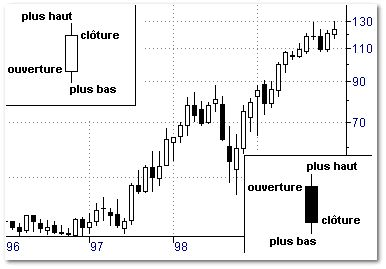
\includegraphics[scale=0.5]{../graph/chandelier.png}
  \caption{Exemple de graphique avec des chandeliers -\url{http://www.abcbourse.com/apprendre}}
\end{figure}

 La désignation pour le chandelier blanc (marché haussier) est le Yang (yo-sen ), pour le chandelier noir (marché baissier) le Yin (in-sen). \\
 
Normalement, après une bougie avec un corps long on ne doit pas prendre position sauf si on est dans un contexte haussier pour une bougie blanche ou contexte baissier pour une bougie noire. 

Pour effectuer des prévisions à partir des chandeliers, il faut être capable de repérer des figures significatives : 
\begin{itemize}
\item  \textbf{Ligne perçante} : représente un retournement. Un long corps de baisse suivi d’un long corps de hausse. Le trait horizontal représente le milieu de la bougie de baisse, la bougie de hausse doit clôturer au-dessus de ce trait.  
\begin{figure}[H]
  \center
  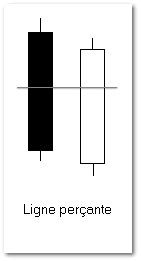
\includegraphics[scale=0.5]{../graph/chandelier1.png}
  \caption{Exemple de ligne perçante - \url{http://www.abcbourse.com/apprendre}}
\end{figure} 

\item \textbf{Ciel ouvert} : condition inverse de la ligne perçante. Un long corps de hausse suivi d’un long corps de baisse. Le corps de baisse ouvre au-dessus du milieu de la bougie de hausse. Ce motif représente un retournement également. 
\begin{figure}[H]
  \center
  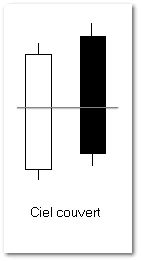
\includegraphics[scale=0.5]{../graph/chandelier2.png}
  \caption{Exemple de ciel ouvert - \url{http://www.abcbourse.com/apprendre}}
\end{figure} 

\item \textbf{Le marteau} : il présage d’une hausse si il arrive au cours d’une baisse. Il n’y a pas d’ombre au dessus et une très longue en dessous, il peut s’agir d’une bougie noire ou blanche la signification est la même .
\begin{figure}[H]
  \center
  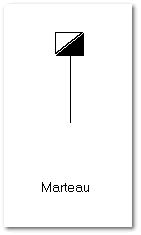
\includegraphics[scale=0.5]{../graph/chandelier3.png}
  \caption{Exemple de marteau - \url{http://www.abcbourse.com/apprendre}}
\end{figure} 

\item \textbf{Le pendu} : il présage d’une baisse si il arrive au cours d’une hausse. Les couleurs n’ont pas d’importance. 
 \begin{figure}[H]
  \center
  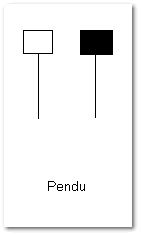
\includegraphics[scale=0.5]{../graph/chandelier4.png}
  \caption{Exemple de pendu - \url{http://www.abcbourse.com/apprendre}}
\end{figure} 

\item \textbf{Les englobantes} : Elles peuvent être haussières ou baissières et sont très puissantes. Si la baissière arrive après une hausse significative ou la haussière après une baisse significative, on assistera probablement à un retournement.
\begin{figure}[H]
  \center
  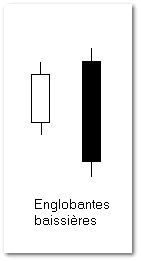
\includegraphics[scale=0.5]{../graph/chandelier5.png}
  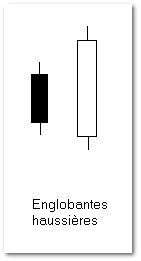
\includegraphics[scale=0.5]{../graph/chandelier6.png}
  \caption{Exemple d'englobante - \url{http://www.abcbourse.com/apprendre}}
\end{figure} 

\item \textbf{Étoile du soir et étoile du matin} : l’étoile du soir indique un retournement possible à la baisse et l’étoile du matin indique au contraire un retournement possible à la hausse.
\begin{figure}[H]
  \center
  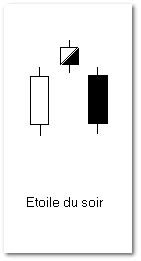
\includegraphics[scale=0.5]{../graph/chandelier7.png}
  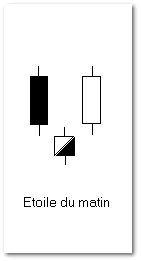
\includegraphics[scale=0.5]{../graph/chandelier8.png}
  \caption{Exemple d'étoile du soir et d'étoile du matin- \url{http://www.abcbourse.com/apprendre}}
\end{figure} 

\item \textbf{Les dojis} : Ils sont très simples à reconnaître : un seul trait horizontal indiquant que les cours de clôtures et d’ouvertures sont les mêmes. Il existe plusieurs types de doji. Le \textbf{doji simple} un long trait vertical de chaque côté de la barre horizontal indique de l’indécision. Les \textbf{dojis dragons}, sont composés d’un long trait sous la barre horizontale, les cours ont beaucoup baissés dans la journée pour se maintenir finalement. Le \textbf{doji pierre tombale} est l’inverse du doji dragon. Si plusieurs dojis se suivent : séance suivante très évolutive.
\begin{figure}[H]
  \center
  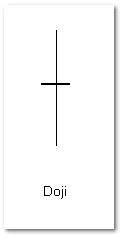
\includegraphics[scale=0.5]{../graph/chandelier9.png}
  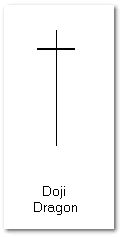
\includegraphics[scale=0.5]{../graph/chandelier10.png}
  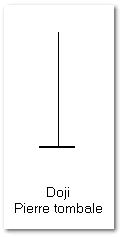
\includegraphics[scale=0.5]{../graph/chandelier11.png}  
  \caption{Exemple de dojis - \url{http://www.abcbourse.com/apprendre}}
\end{figure} 
\end{itemize}

\subsubsection{Les moyennes mobiles}
Les moyennes mobiles sont souvent cités mais pourtant souvent mises au second plan.  La Moyenne Mobile Arithmétique des cours de clôture calculée sur 20 jours, appelée MMA20 se calcule en additionnant les cours des 20 derniers jours et en divisant le résultat par 20. La MMA50, utilise le même principe mais pour 50 jours. Les pics de la courbe des moyennes mobiles sont retardés par rapport à la courbe du cours et sont plus aplatis et arrondis. 

\begin{figure}[H]
  \center
  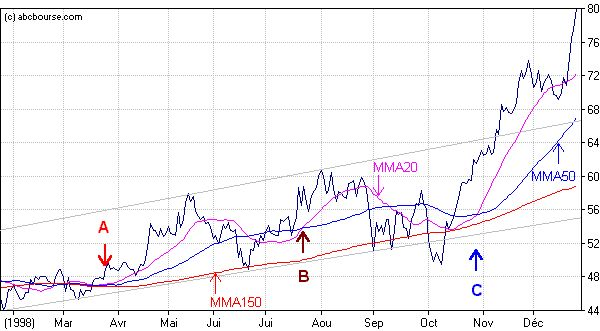
\includegraphics[scale=0.5]{../graph/moyennemobile.png} 
  \caption{Exemple de courbe avec moyenne mobile, en rose MMA20, en bleu MMA50 et en rouge MMA150 - \url{http://www.abcbourse.com/apprendre}}
\end{figure} 

Seule une MMA ne nous donne que très peu d’information, mais en étudiant deux courbes de moyenne mobile on peut en déduire des points intéressants. Lorsque la courbe de la MMA de moyenne la plus courte vient couper la courbe de la MMA de moyenne la plus longue en passant par dessus, la valeur entame un cycle de hausse. Lors d'un croisement entre deux MMAs le gain potentiel est plus fort si l’angle entre les deux MMAs est plus important. \\

Il est conseillé d'effectuer le choix suivant : la MMA de durée longue doit avoir une durée entre deux et quatre fois plus longue que la durée courte, on associe souvent MMA20 et MMA50

Il existe des contre-exemple connus au moyenne mobile :
\begin{itemize}
\item échange de quelques actions par jour seulement, lorsqu'il y a possibilité que les achats par jour puissent faire changer significativement la moyenne mobile de durée courte
\item des actions indépendantes du marché, il ne faut pas prendre MMA20 et MMA50 mais d'autres durée pour coller au titre
\end{itemize}

Il existe d'autres types de moyenne mobile, tels que les Moyennes Mobiles Exponentielles définies par la formule suivante : \\
$MME = Moyennes Mobiles Exponentielles = fermeture du jour * 0.09 + MM de la veille * 0.91$. 


\subsubsection{Les Bandes de Bollinger}
Les Bandes de Bollinger ont été inventées dans les années 80 par John Bollinger. C'est désormais un des indicateurs classiques en analyse technique.  Il sert à évaluer l'évolution future du prix d'un cours. Les Bandes de Bollinger déterminent les niveaux de résistance à la hausse et de support à la baisse. \\

Étudions dans un premier temps la construction des bandes de Bollinger. Dans un premier temps il nous faut une Moyenne Mobile sur n périodes (en général n=20). Cette courbe est appelée la Moyenne Mobile de Bollinger. La Bande Supérieure de Bollinger est calculée de la manière suivante : notre Moyenne Mobile de Bollinger, défini précédemment, plus un nombre x fois écart-types des cours avec cette Moyenne Mobile(en général x=2). La Bande Inférieure de Bollinger est déterminée d'une manière analogue : notre Moyenne Mobile de Bollinger moins x fois écart-types des cours avec cette Moyenne Mobile. \\

L'écart-type est calculé de la manière suivante : $ecartType= \sqrt{\sum{\frac{(cloture-MMS)^2}{n}}} $ \\

Les Bandes de Bollinger sont ainsi deux courbes placées à égales distance de la Moyenne Mobile, elles forment un canal. On peut voir leur représentation sur le schéma suivant, en bleu nous retrouvons la Moyenne Mobile de Bollinger alors qu'en rouge nous retrouvons les deux bandes de Bollinger : 

\begin{figure}[H]
  \center
  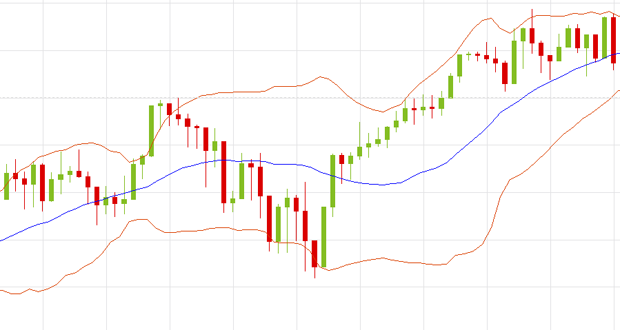
\includegraphics[scale=0.5]{../graph/bollinger.png} 
  \caption{Exemple de bande de Bollinger - \url{https://www.forexagone.com/apprendre/bandes-bollinger}}
\end{figure} 

Maintenant que nous avons défini les Bandes de Bollinger, étudions les informations que nous apportent ces bandes. \\

Première approche avec les Bandes de Bollinger : lorsqu'une tendance est clairement définie, il faut entrer en action lorsque le cours dépassera la bande de Bollinger. Dans le cas d'une tendance haussière, il faudra regarder quand le cours débordera la Bande Supérieure de Bollinger et inversement en tendance baissière il faudra regarder par rapport à la Bande Inférieure de Bollinger. Ainsi dans l'exemple ci-dessous, nous sommes clairement dans le cas d'une tendance baissière. Nous remarquons que le cours franchit trois fois la Bande Inférieure de Bollinger, sur cet exemple il aurait fallu prendre des positions vendeuses à trois reprises. 

\begin{figure}[H]
  \center
  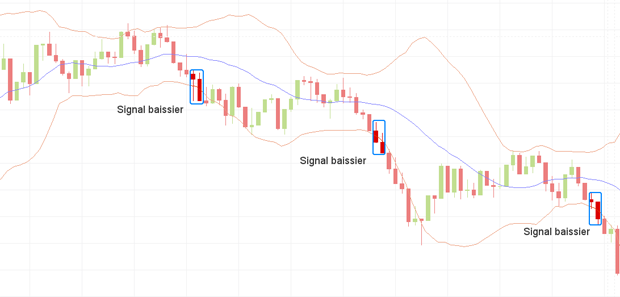
\includegraphics[scale=0.5]{../graph/bollingerBaissier.png} 
  \caption{Exemple de bande de Bollinger en tendance baissière - \url{https://www.forexagone.com/apprendre/bandes-bollinger}}
\end{figure} 
 
 
Deuxième situation : Lorsque le cours n'a pas de tendance clairement défini, il faut faire attention au moment ou le cours croise une Bande de Bollinger. En effet, lorsque le cours croise la Bande Supérieure de Bollinger il faut vendre car les prix vont diminuer et inversement lorsque le cours va toucher la Bande Inférieur il faut acheter. Nous pouvons voir cela sur l'exemple ci-dessous, chaque flèche verte représente un moment où il faut acheter car le cours atteint la Bande Inférieure. Les flèches rouges quand à elles représentent les moments où il faut vendre car le cours atteint la Bande Supérieure.  

\begin{figure}[H]
  \center
  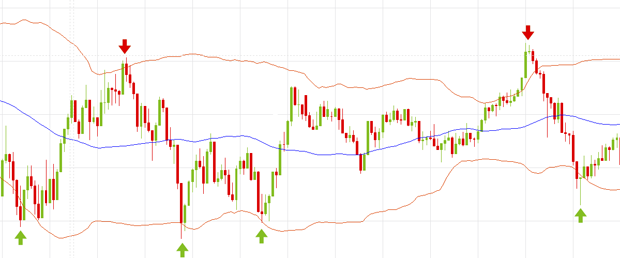
\includegraphics[scale=0.5]{../graph/bollingerRange.png} 
  \caption{Exemple de bande de Bollinger sans tendance - \url{https://www.forexagone.com/apprendre/bandes-bollinger}}
\end{figure} 
 
La dernière situation dans laquelle les Bandes de Bollinger sont utiles est la suivante : lorsque les bandes de Bollinger se ressert très fortement, on appelle cette situation un étranglement. Lorsque l'on est dans le cas d'un étranglement la volatilité des prix est très faible, en effet l'écart-type est très faible ce qui amène le resserrement des deux bandes. Ces phases d'étranglement sont le signe d'une phase d'accélération du cours et donc de volatilité très importante. Les bandes de Bollinger ne nous permettent pas de savoir dans quelle directions les cours vont varier, il faudra dont utiliser d'autres méthodes pour compléter cette analyse et déterminer la tendance qui va suivre. Dans l'exemple ci-dessous nous pouvons remarquer un étranglement dans la zone encadrée en bleue : la volatilité est très faible. Nous savons donc qu'il va y avoir une forte variation du cours à venir. Cela se vérifie lorsque le cours croise la bande inférieure de Bollinger : il s'en suite une chute importante.   

\begin{figure}[H]
  \center
  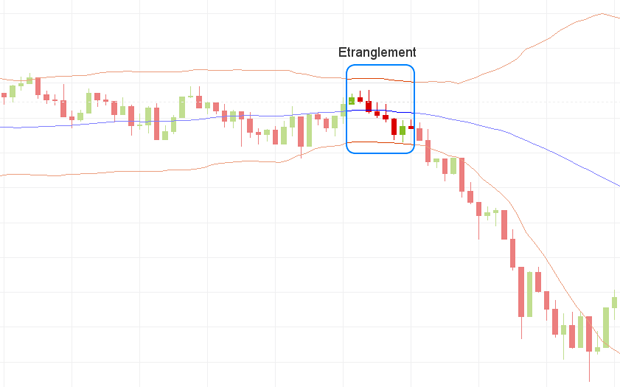
\includegraphics[scale=0.5]{../graph/bollingerEtranglement.png} 
  \caption{Exemple de bande de Bollinger avec étranglement - \url{https://www.forexagone.com/apprendre/bandes-bollinger}}
\end{figure} 
 
Les bandes de Bollinger présente l'avantage d'être très réactif car il sait prévoir les grands changement à venir pour le cours. Néanmoins, il présente l'inconvénient d' évoluer rapidement d'une séance à l'autre. Leur interprétation doit donc être réalisée fréquemment afin d'éviter des erreurs de jugements.  

\subsubsection{Les volumes}


